\section{Geophysics Struct Reference}
\label{struct_geophysics}\index{Geophysics@{Geophysics}}
Collaboration diagram for Geophysics:\begin{figure}[H]
\begin{center}
\leavevmode
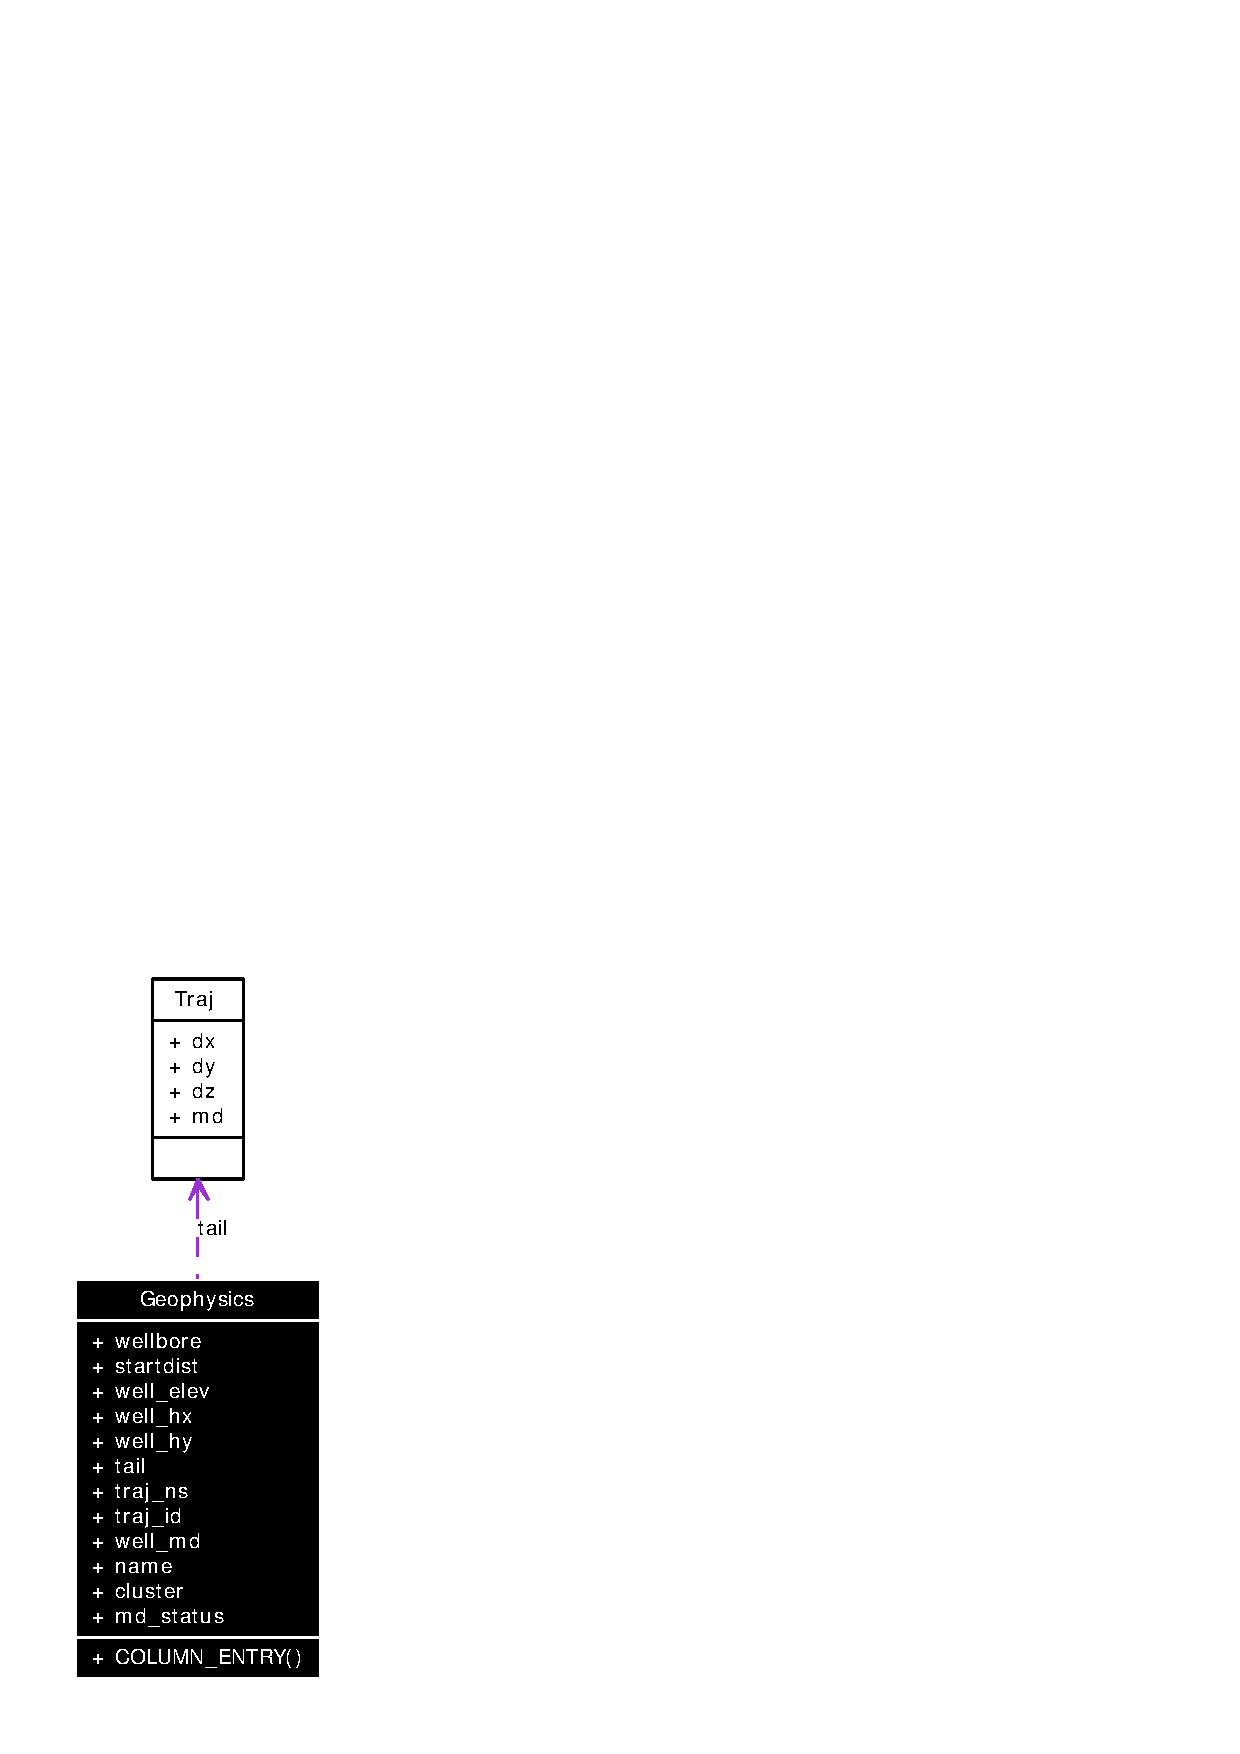
\includegraphics[width=77pt]{struct_geophysics__coll__graph}
\end{center}
\end{figure}
\subsection*{Public Member Functions}
\begin{CompactItemize}
\item 
{\bf COLUMN\_\-ENTRY} (13, {\bf name})\label{struct_geophysics_a0}

\end{CompactItemize}
\subsection*{Public Attributes}
\begin{CompactItemize}
\item 
long {\bf wellbore}\label{struct_geophysics_o0}

\item 
float {\bf startdist}\label{struct_geophysics_o1}

\item 
float {\bf well\_\-elev}\label{struct_geophysics_o2}

\item 
float {\bf well\_\-hx}\label{struct_geophysics_o3}

\item 
float {\bf well\_\-hy}\label{struct_geophysics_o4}

\item 
{\bf Traj} {\bf tail}\label{struct_geophysics_o5}

\item 
short {\bf traj\_\-ns}\label{struct_geophysics_o6}

\item 
unsigned char {\bf traj\_\-id}\label{struct_geophysics_o7}

\item 
float {\bf well\_\-md}\label{struct_geophysics_o8}

\item 
char {\bf name} [32]\label{struct_geophysics_o9}

\item 
long {\bf cluster}\label{struct_geophysics_o10}

\item 
DBSTATUS {\bf md\_\-status}\label{struct_geophysics_o11}

\end{CompactItemize}


\subsection{Detailed Description}




Definition at line 31 of file surface\_\-pick.cpp.

The documentation for this struct was generated from the following file:\begin{CompactItemize}
\item 
surface\_\-pick.cpp\end{CompactItemize}
